\section{Conclusion}
\begin{frame}{Conclusion}
\begin{block}{}
This work is a proposal of an reinforced version of existing PatchCore architecture by replacing the traditional CNN backbone with a Vision-Language Model (VLM) encoder such as CLIP. This reinforcement enables the model to extract semantically rich patch-level features that generalize better across various anomaly types. Moreover, the changes are not only in the encoder itself but also in the inference pipeline with text-guided reasoning, allowing the system to process both visual and semantic data simultaneously: images and natural language queries like "Where is the crack?" or "Is this a burn or a crack?". This approach enables interactive and flexible anomaly detection, bridging the gap between vision models and human semantics.
\end{block}
\end{frame}

\begin{frame}{References}
    \begin{itemize}
        \item Karsten Roth, Latha Pemula, Joaquin Zepeda, Bernhard Schölkopf, Thomas Brox, Peter Gehler. \textit{Towards Total Recall in Industrial Anomaly Detection}. CVPR 2021. 
        \item \url{https://github.com/amazon-science/patchcore-inspection}
    \end{itemize}
\end{frame}

\begin{frame}{Further Questions}
    \begin{block}{Which VLM model is used in this context?}
    \begin{itemize}
        \item CLIP can be chosen, especially with its pre-trained variants ViT-L/14
    \end{itemize}
    \end{block}
\end{frame}

\begin{frame}{Further Questions}
    \begin{block}{Does the VLM just replace the pretrained encoder mechanically, or connect with existing PathCore blocks?}
    \begin{itemize}
        \item Combine VLM encoder with CNN backbone for better anomaly detection:
        \begin{itemize}
            \item Keep low-level CNN features (local texture patterns, edges, fine defects).
            \item Add high-level VLM features (semantic, global context).
        \end{itemize}
    \end{itemize}
    \end{block}
\end{frame}
\begin{frame}{New Structure}
    \begin{figure}
        \centering
        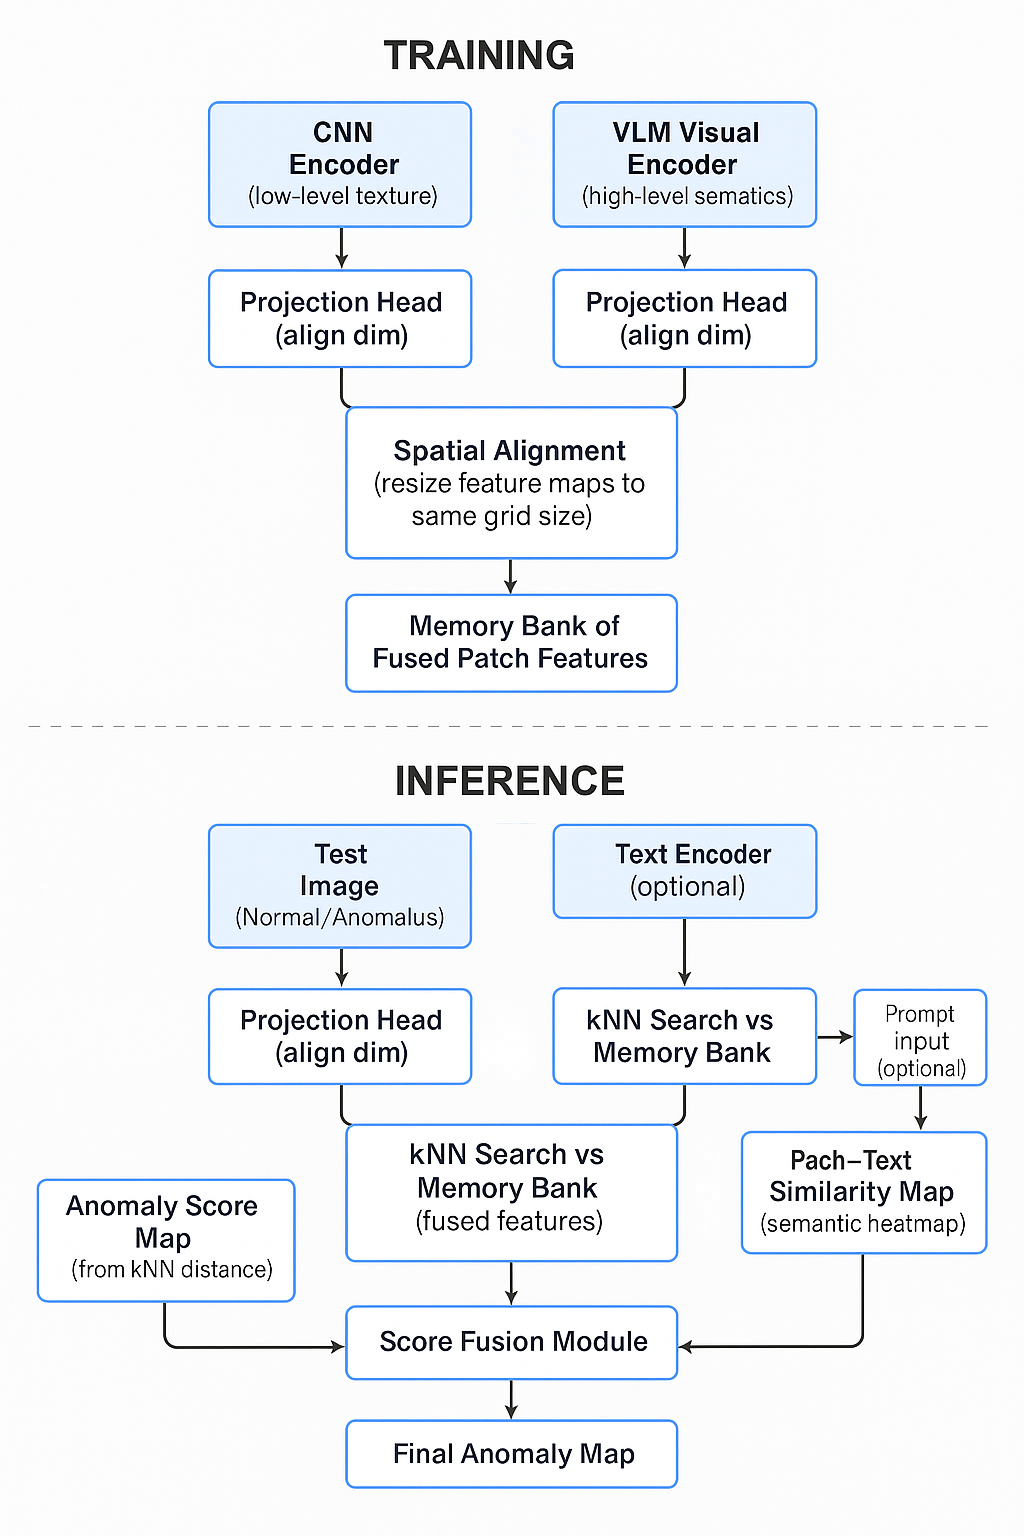
\includegraphics[width=0.33\linewidth]{images/9f58aabd-d1da-426d-9bd9-7c6cf98569a8.png}
    \end{figure}
\end{frame}
\begin{frame}{Further Questions}
    \begin{block}{Should there be additional blocks in PatchCore when adding a VLM?}
    \begin{itemize}
        \item Yes, there should be  more blocks added to this structure:
        \begin{itemize}
            \item VLM visual encoder
            \item Projection heads (CNN \& VLM)
            \item Fusion module
            \item Dimensionality reduction / normalization
            \item Text encoder & prompt processor for interference
            \item Score fusion module
            \item Efficient search index (FAISS)
        \end{itemize}
    \end{itemize}
    \end{block}
\end{frame}

\begin{frame}{Further Questions}
    \begin{block}{Does the VLM need pre-training?}
        \begin{itemize}
            \item This new PatchCore structure will use CLIP as encoder, which is already pre-trained on massive datasets to have general-purpose visual-semantic knowledge.
            \item Only new components like Projection heads  and Fusion module need traing in order to respectively align CNN & VLM features to same dimension and combine aligned CNN (texture) and VLM (semantic) features into one rich representation.
        \end{itemize}
    \end{block}
\end{frame}

\begin{frame}{Further Questions}
\begin{block}{Does the memory bank change after adding VLM? Impact on clustering & coreset?}
    \begin{itemize}
        \item Memory bank now stores fused patch embeddings (or can be separated into two linked banks: CNN-bank and VLM-bank). Fused vectors likely have higher dimension and encode both texture + semantics.
        \item Possible effects:
        \begin{itemize}
            \item Positive: better semantic grouping and localization
            \item Risks: storage increase leads to larger memory and slower progress along with risk of losing tiny anomalies.
        \end{itemize}
        \item Potential solutions: Dim. reduction, dual-bank of VLM and CNN, stratified coreset
    \end{itemize}
\end{block}
\end{frame}